%  !TeX  root  =  user_guide.tex

\chapter{Работа с растровыми данными}\label{label_raster}
\index{raster layers|(}

% when the revision of a section has been finalized,
% comment out the following line:
%\updatedisclaimer

В этом разделе описывается, как отобразить и установить свойства
растрового слоя. QGIS поддерживает множество различных форматов.
В настоящее время протестированы следующие форматы:\index{raster layers!data formats}

\begin{itemize}[label=--]
\item Arc/Info Binary Grid
\item Arc/Info ASCII Grid
\item GRASS Raster
\item GeoTIFF
\item JPEG
\item Spatial Data Transfer Standard Grids (с некоторыми ограничениями)
\item USGS ASCII DEM
\item Erdas Imagine
\end{itemize}

Поскольку реализация растра в QGIS основана на библиотеке GDAL, то,
возможно, и другие форматы растров, основанных на GDAL, будут работать.
В случае сомнения, можно попытаться открыть растр и посмотреть,
поддерживается ли он в QGIS. Больше информации о поддержке растровых
форматов GDAL в Приложении~\ref{appdx_gdal}
\index{raster layers!GDAL implementation}
или на  \url{http://www.gdal.org/formats_list.html}. Если вы хотите
загрузить растровые данные формата GRASS, то обратитесь к
Разделу~\ref{sec:load_grassdata}.

\section{Что такое растровые данные?}\label{label_whatsraster}
\index{raster layers!definition}

Растровые данные в ГИС представляют из себя матрицы, где каждая ячейка
передает значение некого параметра поверхности. Каждая ячейка в
растровой сетке имеет определенный размер. Обычно, они имеют
прямоугольную форму (в QGIS они всегда прямоугольные).  Типичный набор
растровых данных включает в себя данные дистанционного зондирования
такие как аэрофотосъемка, спутниковые снимки или смоделированные данные,
например матрицу высот.

В отличии от векторных данных, у растров, как правило, нет присоединенной
информации к каждой ячейке. Они геокодируются размещением пикселей
относительно координат углового пикселя растрового слоя Это позволяет
QGIS корректно размещать данные на карте.

QGIS использует информацию о геопривязке, находящуюся внутри растрового
слоя (например, GeoTiff) или в соответствующем файле регистрации для
правильного отображения данных.\index{raster layers!georeferenced}

\section{Загрузка растровых данных в QGIS}\label{label_loadraster}

Растровые слои загружаются нажатием на кнопку
\toolbtntwo{mActionAddRasterLayer}{Загрузить растр} или выбором меню
\mainmenuopt{Вид} >
\dropmenuopttwo{mActionAddRasterLayer}{Добавить растроый слой}.
Несколько слоев можно загрузить, удерживая клавишу \keystroke{Control}
или \keystroke{Shift} в диалоге \dialog{Добавить растровый слой}.\index{raster layers!loading}

Когда растровый слой загрузился в окно <<Слои>>, нажмите на нем правой
кнопкой мыши для вызова контекстного меню.

\minisec{Контекстное меню для растровых слоев}

\begin{itemize}[label=--]
\item \dropmenuopt{Увеличить до границ слоя}
\item \dropmenuopt{Увеличить до наилучшего масштаба (100\%)}
\item \dropmenuopt{Показать в обзоре}
\item \dropmenuopt{Удалить}
\item \dropmenuopt{Свойства}
\item \dropmenuopt{Переименовать}
\item \dropmenuopt{Добавить группу}
\item \dropmenuopt{Развернуть все}
\item \dropmenuopt{Свернуть все}
% \item \dropmenuopt{Show file groups} - такого нет.
\end{itemize}

\section{Свойства растра}\label{label_rasterprop}

Чтобы показать и установить свойства растрового слоя необходимо два раза
кликнуть на нем мышкой в окне <<Слои>> или нажать на растре правой
кнопкой мыши и выбрать \dropmenuopt{Свойства} из контекстного
меню:\index{raster layers!context menu}. На рисунке~\ref{fig:raster_properties}
показанано диалоговое окно \dialog{Свойства слоя}. Оно состоит из
вкладок:

\begin{itemize}[label=--]
 \item \tab{Символика}
 \item \tab{Прозрачность}
 \item \tab{Цветовая карта}
 \item \tab{Общие}
 \item \tab{Метаданные}
 \item \tab{Пирамиды}
 \item \tab{Гистограммы}
\end{itemize}

\begin{figure}[h]
  \centering
   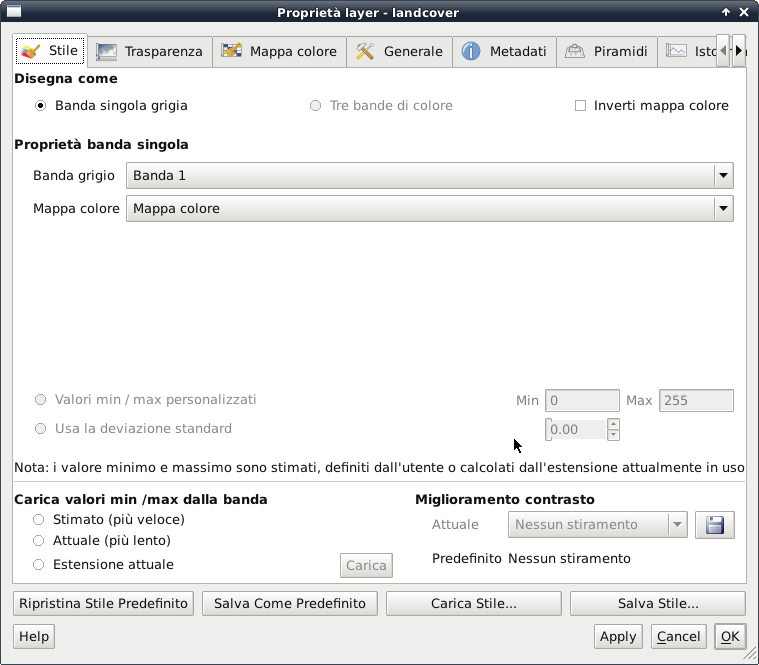
\includegraphics[clip=true, width=14cm]{rasterPropertiesDialog}
   \caption{Свойства слоя \nixcaption}\label{fig:raster_properties}
\end{figure}

\subsection{Символика}\label{label_symbology}

QGIS может отображать растровые слои в двух видах:\index{raster layers!supported channels}

\begin{itemize}[label=--]
\item Одноканальный серый --- изображение будет показано в сером цвете
или в псевдоцветном. % еще в кислотном и цветовой картой
\item Трехканальное цветное --- растр отображается в виде трех каналов:
красный, зеленый и синий, которые используются для создания цветного
изображения.
\end{itemize}

В обоих типах отображения можно инвертировать цвета, используя флажок
\checkbox{Обратить цветовую карту}. %может лучше "гамму"?

\minisec{Одноканальное отображение}

Этот режим предлагает из двух опций. Первая --- выбор канала, который
нужно отобразить (если данные состоят из нескольких каналов).

Вторая --- выбор имеющихся цветовых схем для отображения.

В выпадающем списке доступны следующие настройки:
\selectstring{{}Цветовая карта}{Градация серого} --- градации серого
установлены по умолчанию. Также доступны
\begin{itemize}[label=--]
\item Псевдоцвет
\item Кислотная
\item Цветовая карта
\end{itemize}

При выборе \selectstring{{}Цветовая карта}{Цветовая карта}, становится
доступной вкладка \tab{Цветовая карта}. Подробнее в разделе~\ref{label_colormaptab}.

QGIS может скрывать пиксели, чьи значения находятся вне заданного
интервала стандартных отклонений от среднего по слою.\index{raster layers!standard deviation}
Это полезно тогда, когда в растровой сетке присутствуют одна или две ячейки
с завышенными значениями и которые негатино влияют на отображение растра.
Эта опция доступна только для изображений в псевдоцвете.

\minisec{Трехканальное отображение}

Этот режим позволяет более гибко изменять внешний вид растрового слоя. % appereance - ошибка в оригинале; нужно "appearance"
Например, можно изменить цветовые каналы со стандартной RGB-схемы на
какие-нибудь другие.

Также доступны и диапозоны цветов.


\begin{Tip}\caption{\textsc{Просмотр одного канала многоканального растра}}
Если нужно отобразить только один канал (например, красный) в
многокальном изображении, то нужно выставить каналы зеленый и синий как
<<Не задано>>. Но это не совсем корректно. Для отображения красного
канала нужно выставить тип отображения как градации серого, а затем
выбрать красный как основной канал для серого.
\end{Tip}

\subsection{Прозрачность} \label{rastertab:transparency}

QGIS имеет возможность отображать растровые слои с разной степенью
прозрачности.\index{raster layers!transparency} Для этого используется
ползунок прозрачности, с помощью которого можно указать, до какой
степени слой может быть прозрачным, чтобы увидеть слои, находящиеся под
ним. Это очень удобно, когда загружено множество растровых слоев,
например растр с изображением рельефа и основной растр. Это позволит
сделать внешний вид карты более трехмерным.

Также, можно ввести величину растра, которая будет рассматриваться
как {\em NODATA}.

Более гибко степень прозрачности можно настроить во вкладке
\guiheading{Добавить значения вручную}. В ней можно установить
прозрачность каждого пикселя.

Например, нужно установить прозрачность воды в растре
\filename{landcover.tif} 20\%. Для этого нужно:
\begin{enumerate}
 \item  Загрузить растр \filename{landcover}
 \item Открыть \dialog{Свойства} растра кликнув по нему два раза или
 кликнуть на нем правой кнопкой мыши и выбрать \dropmenuopt{Свойства}
 из контекстного меню.
 \item Выбрать вкладку \tab{Прозрачность}
 \item \label{enum:add} Нажать кнопку
 \toolbtntwo{mActionNewAttribute}{Добавить значения вручную}. Появится
 новая строка в перечне прозрачных пикселей
 \item \label{enum:transp} Ввести значения растра (например, 0) и
 установить прозрачность на 20\%
 \item Нажать \button{Применить} и посмотреть результат на карте
\end{enumerate}

Можно повторить шаги \ref{enum:add} и \ref{enum:transp} чтобы добавить
больше значений для задания прозрачности.

Как можно видеть, выставление прозрачности растра"--- это просто. Но
требует небольших затрат времени. Чтобы быстрее выставлять прозрачность
растра можно воспользоваться кнопкой
\toolbtntwo{mActionFileSave}{Экспорт в файл} для сохранения заданных
настроек. Кнопка \toolbtntwo{mActionAddRasterLayer}{Импорт из файла}
загружает сохраненные ранее настройки прозрачности и применяет их к
выбранному растровому слою.

\subsection{Цветовая карта} \label{label_colormaptab}
% FIXME: Write me

Вкладка \tab{Цветовая карта} доступна при выборе одноканального режима
отображения растра во вкладке \tab{Символика} (см. главу~\ref{label_symbology}).

Доступны три вида интерполяции цветов:
\begin{itemize}[label=--]
\item Дискретная
\item Линейная
\item Точечная
\end{itemize}

Кнопка \button{Добавить значение} добавляет цвет в пользовательское
значение цветовой карты. Двойной щелчок мыши на поле <<Значение>>
позволяет задать конкрентую величину. Двойной щелчок мыши на поле
<<Цвет>> открывает диалоговое окно \dialog{Выбор цвета}, в котором
можно выбрать цвет для заданной величины.

Или же можно нажать на кнопку
\toolbtntwo{mActionNewAttribute}{Загрузить цветовую карту из канала},
которая загружает таблицу из канала (если она в нем присутствует).

Блок \guiheading{Создать новую цветовую карту} позволяет создавать
новые категории цветовой карты. Для этого задается нужное
\selectnumber{{}количество значений}{15} и нажимается кнопка
\button{Классифицировать}. В настоящее время поддерживается только
\selectstring{{}Режим классификации}{Равные интервалы}\index{raster layer!classify}.

\subsection{Общие}\label{label_generaltab}

Вкладка \tab{Общие} отображает основную информацию выбранного растра,
в том числе источник слоя и его имя в легенде (которое можно изменить).
Также, в этой вкладке отображается образец слоя, его легенда и палитра.\index{raster layers!properties}

Кроме того, в этой вкладке можно установить видимость слоя в пределах
масштаба. Для этого нужно установить флажок в соответствующем поле и
задать масштаб, в пределах которого данный слой будет отображаться на
карте.

Также здесь отображается система коородинат в виде строки PROJ.4. Ее
можно изменить, нажав кнопку \button{Выбрать}.

\subsection{Метаданные}\label{label_metatab}

Вкладка \tab{Метаданные} отображает полные данные о растровом слое,
включая статистику о каждом канале загруженного растра. Статистические
данные собираются по принципу <<нужно знать>>, так что, возможно,
статистика по слоям может быть не доступной.\index{raster layers!metadata}

В основном, эта вкладка используется для просмотра информации. В ней
нельзя изменить какие-либо значения. Для обновления статистики нужно
перейти на вкладку \tab{Гистограмма} и нажать кнопку \button{Обновить}.
Подробнее в главе~\ref{label_histogram}.

\subsection{Пирамиды}\label{raster_pyramids}

Растры высокого разрешения могут замедлить навигацию в QGIS. Создание
копий данных низкого разрешения (пирамид) позволяет существенно повысить
скорость, поскольку QGIS будет автоматически выбирать оптимальное
разрешение в зависимости от текущего масштаба.
\index{raster layers!pyramids}
\index{raster layers!resolution pyramids}

Для сохранения пирамид необходимы права на запись в каталог, в котором
хранятся оригинальные данные. \\
Для построения пирамид используются два метода интерполяции:
\begin{itemize}[label=--]
\item Среднее значение
\item Ближайший сосед
\end{itemize}

Если поставлен флажок
\checkbox{Создавать встроенные пирамиды, если возможно} QGIS будет
пытаться создать внутренние пирамиды.

Обратите внимание, что операция построения встроенных пирамид может
изменить оригинальный файл данных и их невозможно будет удалить после
создания. Поэтому желательно создавать резервную копию растра перед этой
операцией.

\subsection{Гистограмма}\label{label_histogram}

Вкладка \tab{Гистограмма} позволяет просмотреть распределение \index{raster layers!histogram}
каналов или цветов в растре. Для начала нужно создать статистику растра,
нажав на кнопку \button{Обновить}. Можно выбрать отдельные каналы для
отображения из списка. Доступно два вида диаграмм:

\begin{itemize}[label=--]
\item Столбчатая
\item Линейная
\end{itemize}

Также, можно задать количество столбцов диаграммы и режим отображения:
\checkbox{Разрешить аппроксимацию} или \checkbox{Разрешить значения вне диапозона}.
После просмотра гистограммы можно заметить, что поля статистики каналов
на вкладке \tab{Метаданные} будут заполнены.\index{raster layers!metadata)}

\begin{Tip}\caption{\textsc{Сбор статистики растра}}
Для сбора статистики по слою, выберите псевдоцветное преобразование и
нажмите \button{Применить}. Сбор статистики может занять продолжительное
время. Пожалуйста, будте терпиливы, пока QGIS обработает выши данные!\index{raster layers!statistics}
\end{Tip}

\FloatBarrier
